%preamble
\documentclass[letterpaper]{article}
\synctex=1
\usepackage{graphicx}
\graphicspath{ {images/} }

\usepackage{lipsum}
\usepackage{float}
% \bibliographystyle{IEEEtran}
% \bibliographystyle{ieeetr}

\usepackage{amssymb}

\usepackage{siunitx}

\usepackage{multirow}
% for merging table cells I think

\usepackage{tabularx}
% allows for linewrap within cells
\newcolumntype{Y}{>{\centering\arraybackslash}X}

\usepackage{todonotes}

% \usepackage[utf8]{inputenc}
% \usepackage[russian]{babel}
% WHY CAN'T I USE є IN MATH MODE
% \usepackage[T2A,T1]{fontenc}
% \DeclareSymbolFont{cyrillic}{T2A}{cmr}{m}{n}
% \DeclareMathSymbol{\Sha}{\mathalpha}{cyrillic}{216}
% \DeclareMathSymbol{\cyrje}{\LastDeclaredEncoding}{106}

\usepackage{fancyhdr} %header
\fancyhf{}
\fancyhead[R]{Arun Woosaree XXXXXXX}
\renewcommand\headrulewidth{0pt}
\fancyfoot[C]{\thepage}
\renewcommand\footrulewidth{0pt}
\pagestyle{fancy}

% make subsection use letters
\renewcommand{\thesubsection}{\thesection\ \alph{subsection})}


% \usepackage{amsthm}

%actual document
\begin{document}

% \maketitle %insert titlepage here
\begin{titlepage}
 \begin{center}
  \vspace*{1cm}
  \Huge
  Stat 235
  \vspace{1cm}
  
  Lab 5
  \vspace{1cm}
  
  WOOSAREE, Arun
  \vspace{1cm}
  
  \Huge
  Lab EL12
  \vspace{1cm}
  
  TA: Jessa Marley
  \vspace{1cm}
  
  \today
  \vfill
 \end{center}
\end{titlepage}

\section{1.	First examine the relationship between the response variable (thrust) and each of of the three  predictor variables with scatterplots.}
\label{q1}

\subsection{(a)	Obtain a scatterplot of thrust versus each of the three predictors. The  format of each of the three scatterplots should be consistent with the format used in Lab 1 Instructions (no lines or grids, axes rescaled to display only the observed values, title, names of the axes).  Paste the three scatterplots into your report. }
OUTPUT: 3 Scatterplots, thrust vs. Fuel flow rate, thrust vs.
exhaust temperature, thrust vs. Ambient temperature.
What should be on the y-axis?
\todo{captions}
\begin{figure}[H]
 \centering
 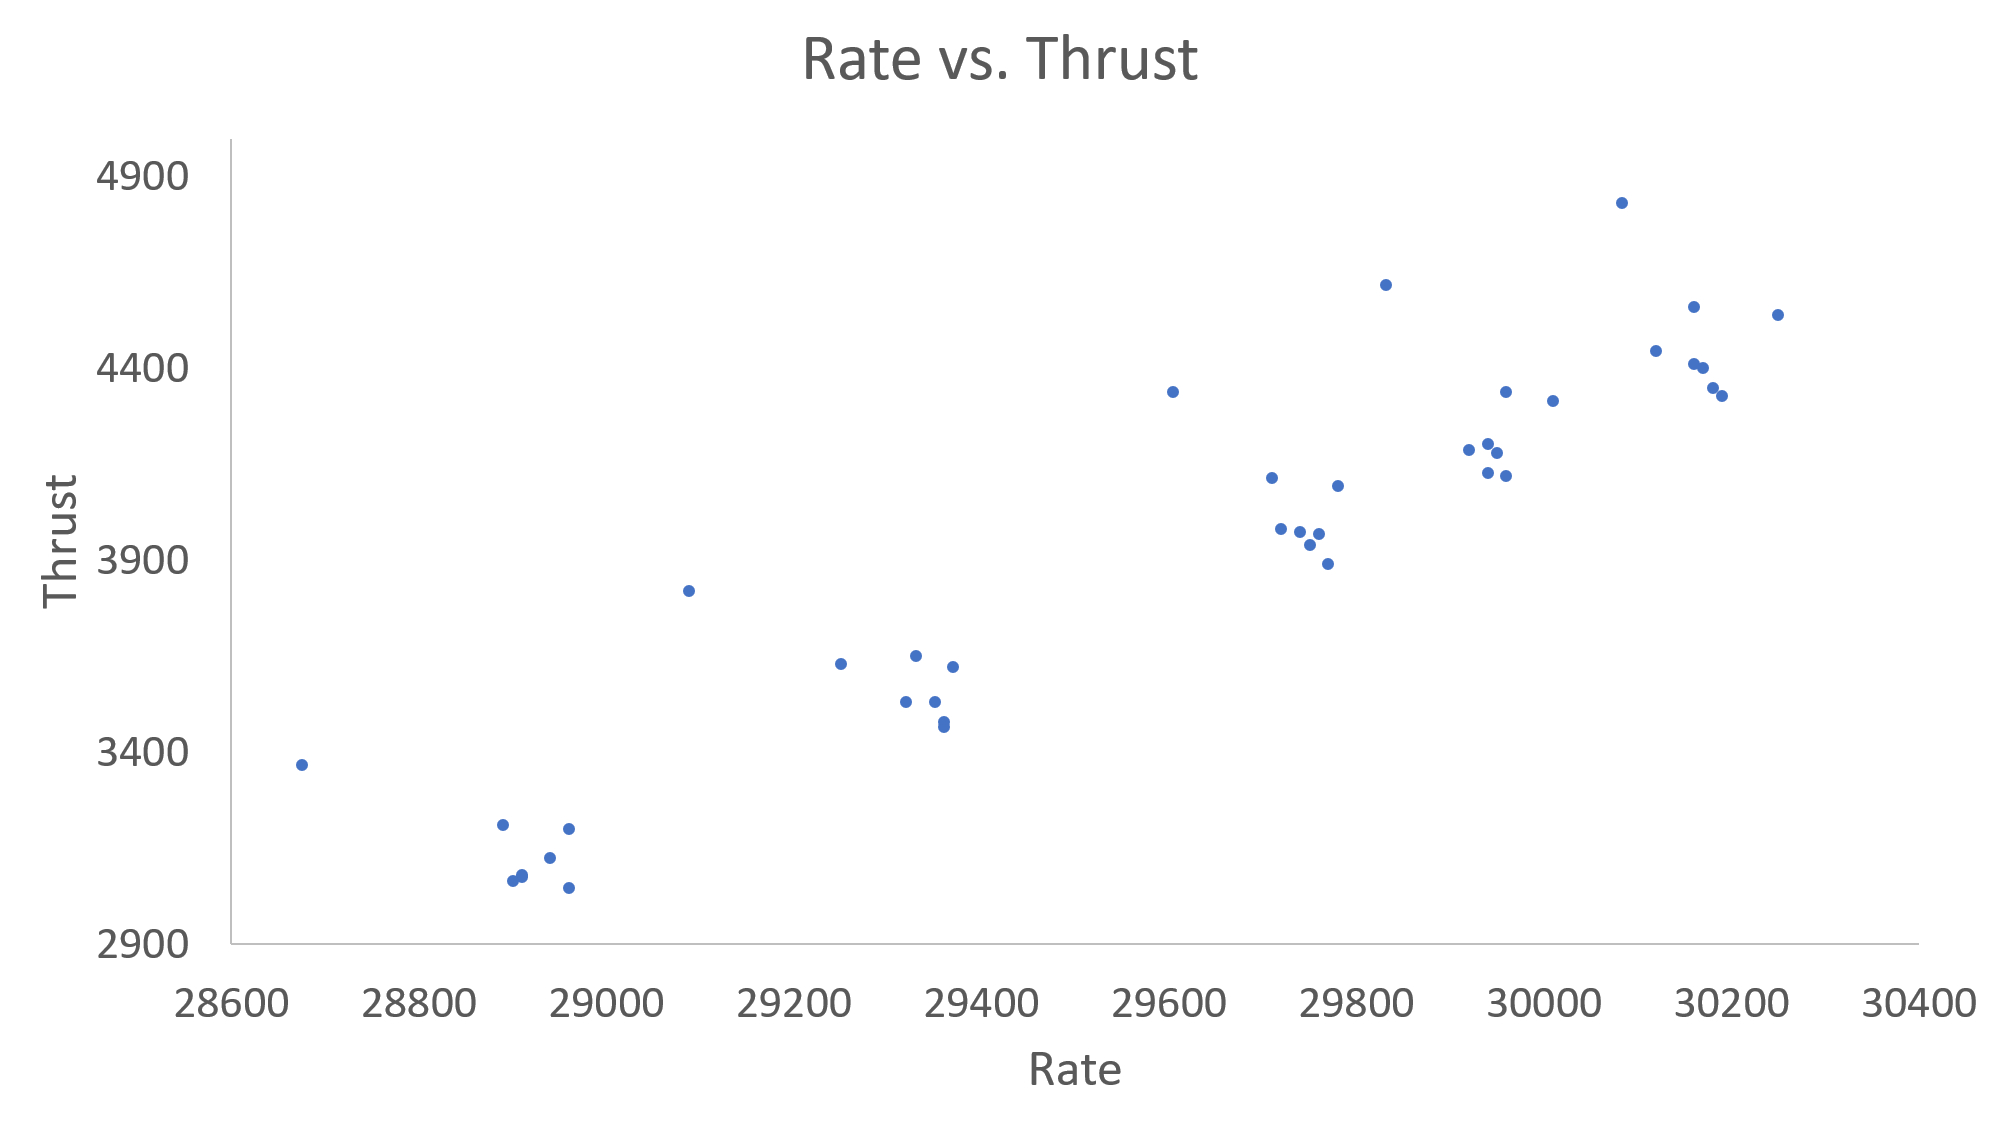
\includegraphics[width=\textwidth]{ratethrust.png}
 \caption{INSERT CAPTION HERE}
 \label{ratethrust}
\end{figure}

\begin{figure}[H]
 \centering
 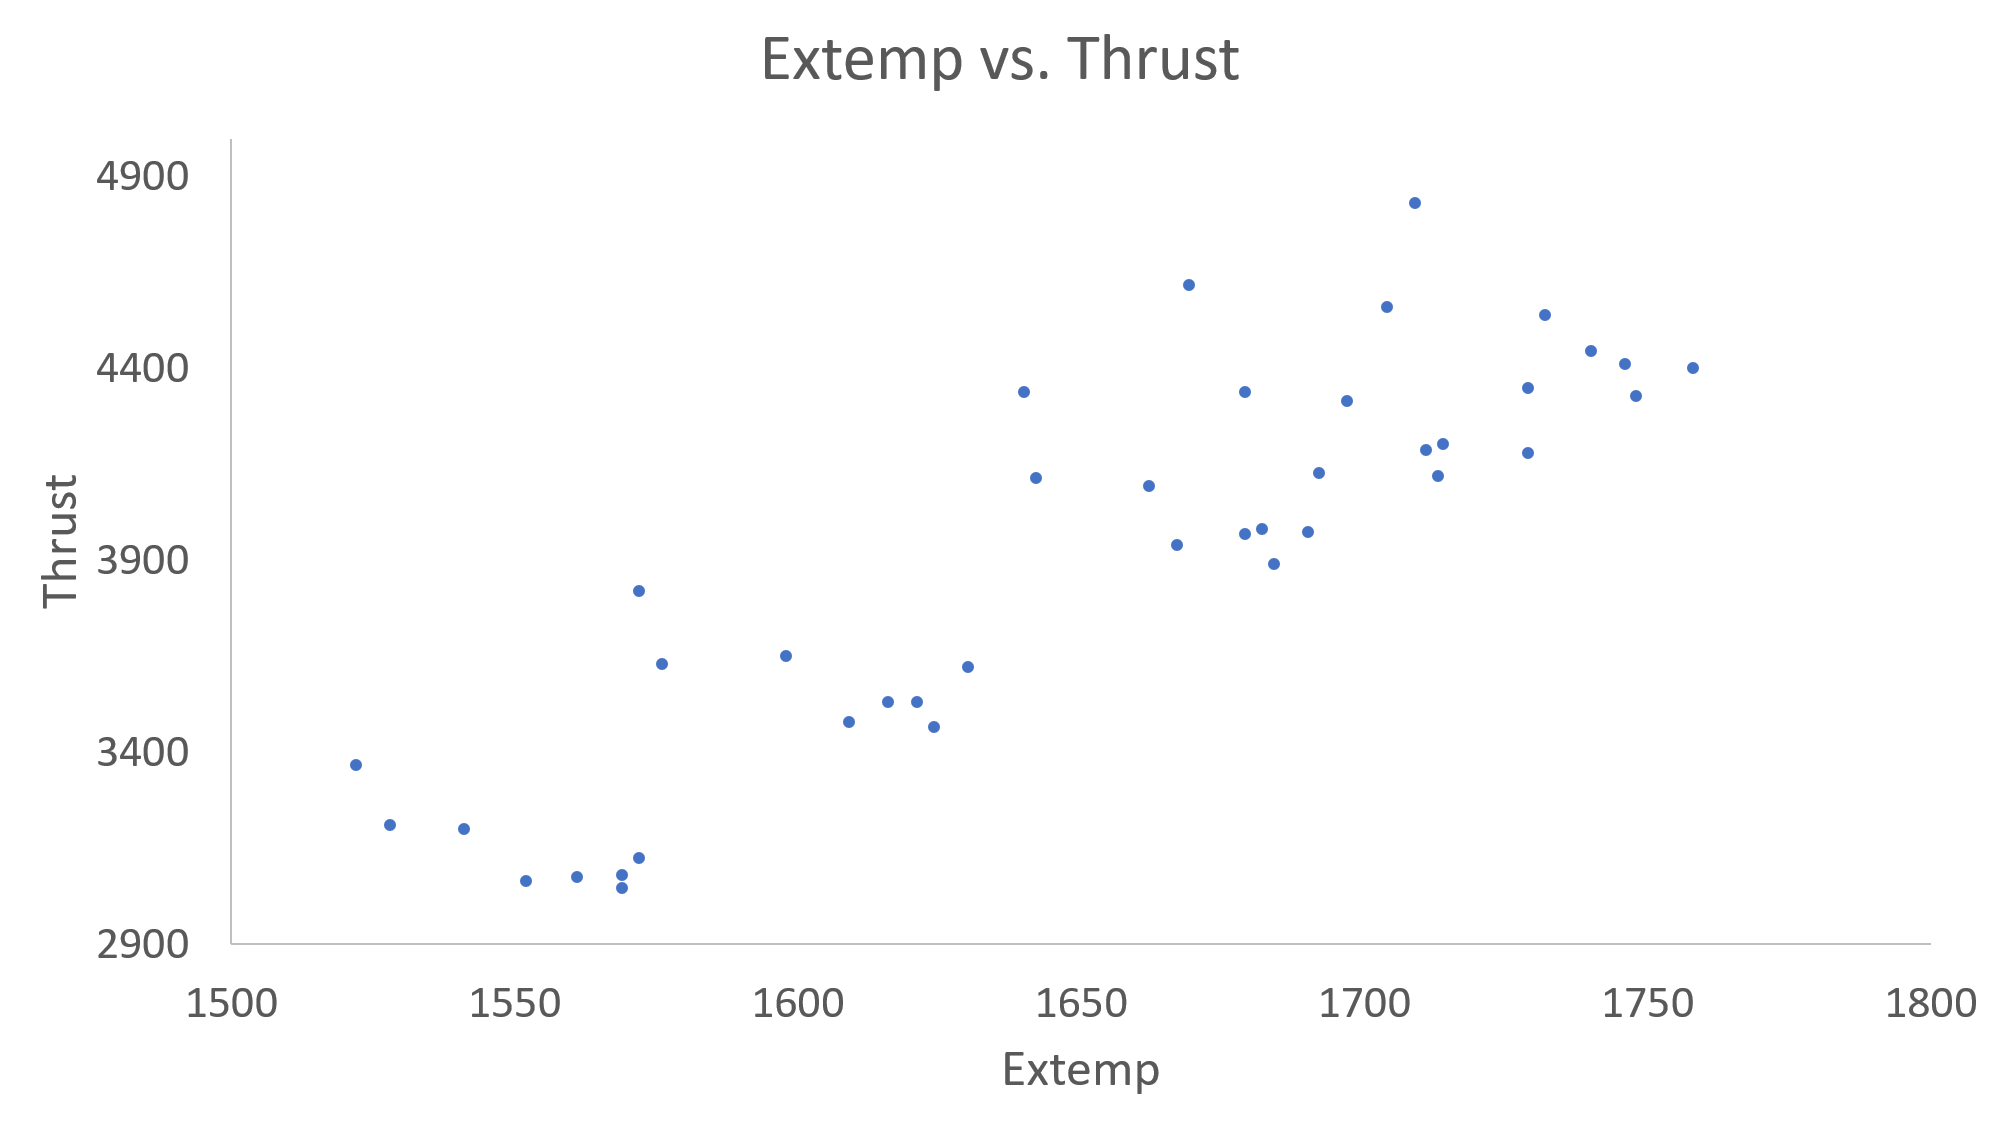
\includegraphics[width=\textwidth]{extempthrust.png}
 \caption{INSERT CAPTION}
 % \label{q6}
\end{figure}

\begin{figure}[H]
 \centering
 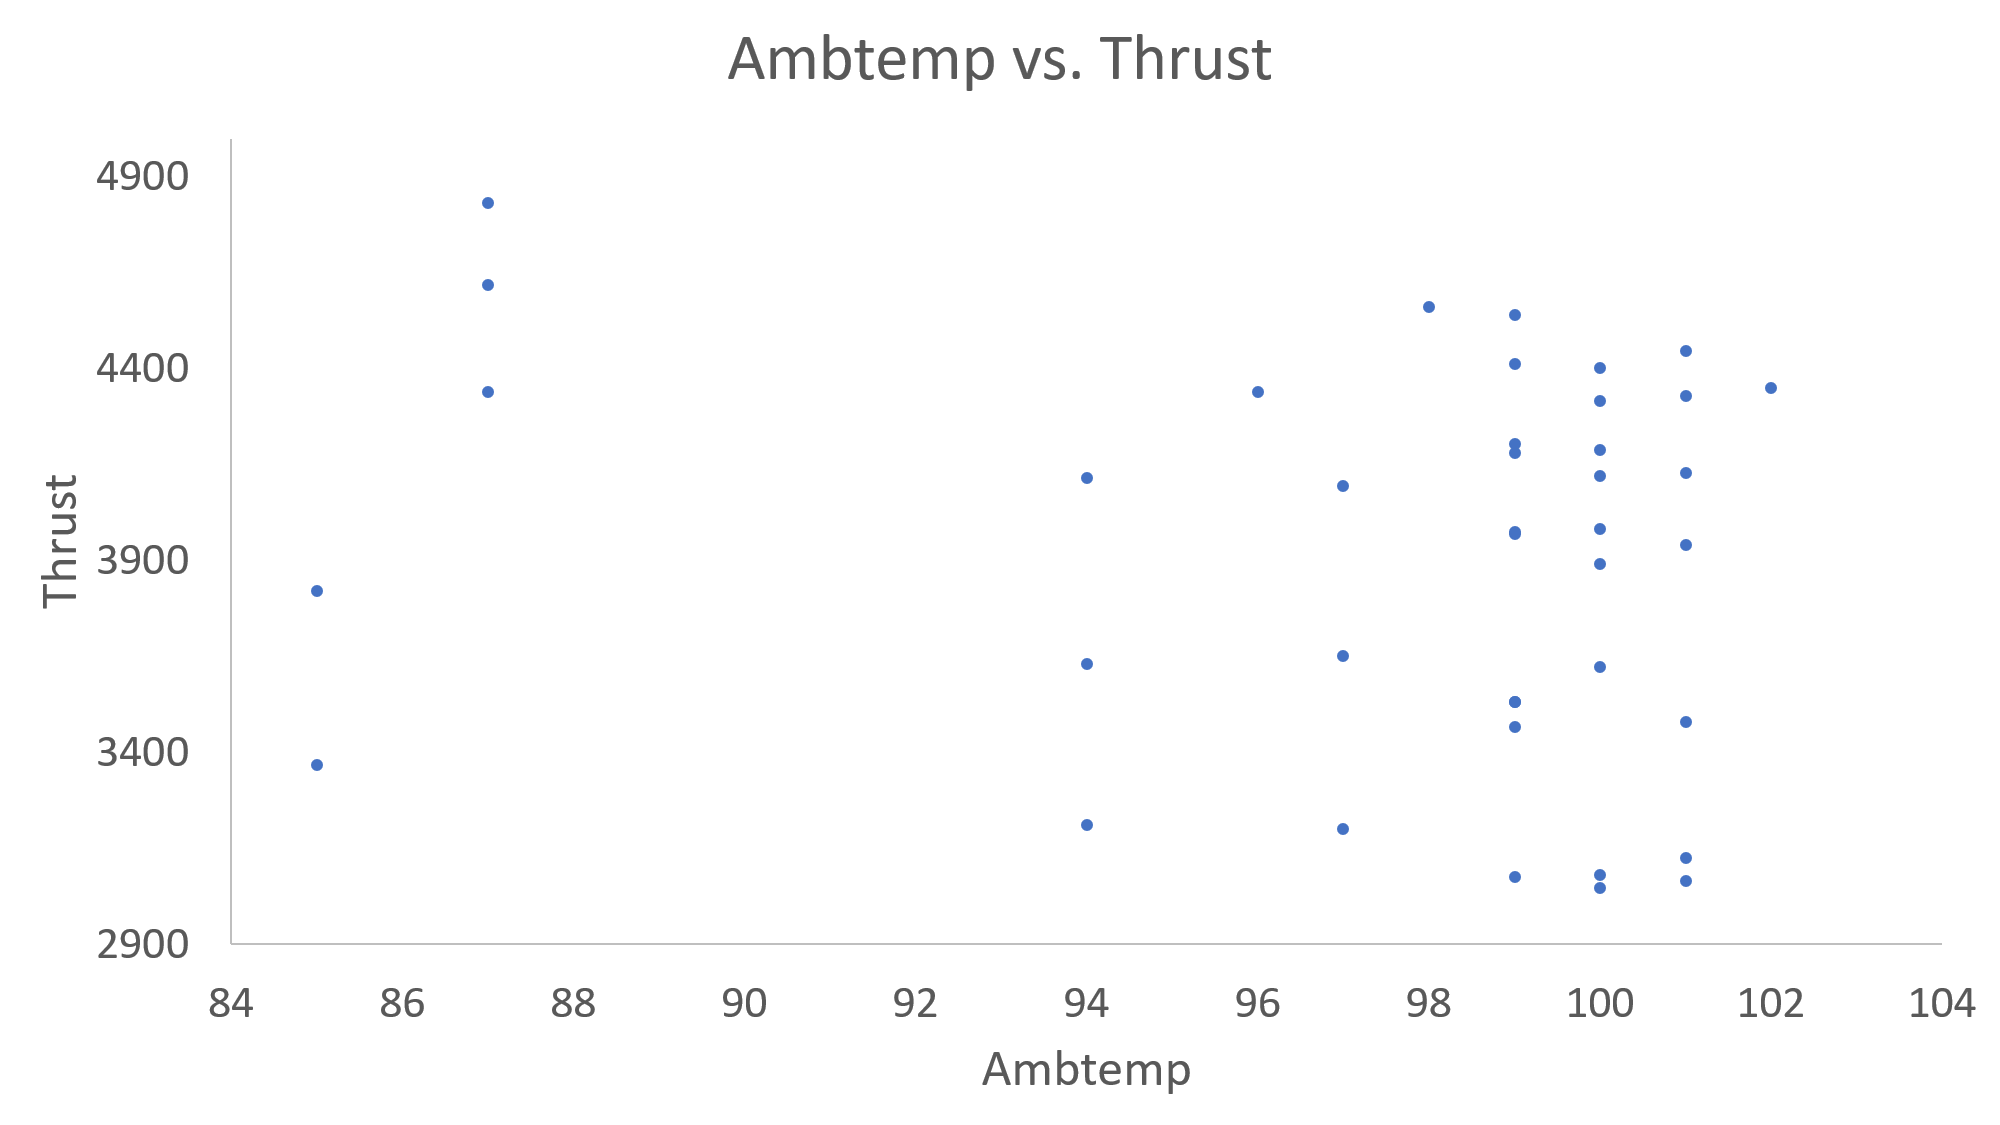
\includegraphics[width=\textwidth]{ambtempthrust.png}
 \caption{INSERT}
 % \label{q6}
\end{figure}

\subsection{(b)	Comment briefly on the relationship between thrust and each of the three predictors. In particular, comment on the overall shape (line, curve), direction (positive, negative), and strength (size of the scatter and its inclination) of the relationship. Which of the three predictor variables seems to be the best predictor of thrust? }
\label{1b}
Look at the center of the “clouds”.  Are they linear? Strength of
linear relationship?

\begin{itemize}
 \item The plot for rate vs. thrust above appears to exhibit a relatively strong positive
       linear relationship, with less scatter relative to the other plots.
 \item The plot for extemp vs. thrust above appears to exhibit a fairly strong positive
       linear relationship, but with a bit more scatter than Figure \ref{ratethrust}.
 \item The plot for ambtemp vs. thrust above does not appear to exhibit a strong linear
       relationship due to the points being very visually scattered.
       If there is a linear relationship, it looks like it would be almost flat,
       with a slightly negative slope.
\end{itemize}

Overall, the rate seems to have the stongest linear relationship with the thrust,
since it has a positive slope and the least amount of scatter.
\todo{Which of the three predictor variables seems to be the best predictor of thrust?}
So it's the best predictor?

\section{2.	Examining the array of all possible pairwise correlation coefficients is another way to understand the relationships among variables. Use the Correlation tool in the Data Analysis menu to obtain the correlation matrix for the four variables}

\subsection{(a)	Paste the correlation matrix into your report. Make sure that the matrix contains the names of all variables.}
OUTPUT: Correlation matrix.

\begin{table}[H]
 \centering
 \begin{tabular}{c|c|c|c|c|}
          & rate        & extemp      & ambtemp  & thrust \\ \hline
  rate    & 1           &             &          &        \\ \hline
  extemp  & 0.975750317 & 1           &          &        \\ \hline
  ambtemp & 0.216465939 & 0.301764125 & 1        &        \\ \hline
  thrust  & 0.928792499 & 0.87169251  & -0.14744 & 1      \\ \hline
 \end{tabular}
 \caption{Correlation matrix}
 \label{correlationmatrix}
\end{table}
\todo{caption}

\subsection{(b)	Identify the regressor variables (predictors) having the largest and smallest absolute values of correlation with the response variable (thrust). Do the signs and magnitudes of the correlation coefficient between thrust and each predictor confirm your conclusions you have reached in Question 1? Explain briefly.}
Highest correlation, lowest (note absolute value)? Does this
match the conclusions from Q1?

The regressor variable with the largest magnitude of correlation with the response
variable thrust is the rate, with a value of $0.928792499$.
The regressor variable with the lowest magnitude of correlation with the thrust
is ambtemp, with a value of $-0.14744$.
The values obtained in Table \ref{correlationmatrix} agree
with the conclusions reached in Question \ref{q1}, with
the rate having the largest correlation with a positive slope, and the
ambient temperature having a weak correlation and slightly negative slope.
Additionally, we see that the external temperature also has a fairly strong
linear relation with the thrust, and its correlation value is both positive and less than
the rate variable, as predicted in Question \ref{1b}.
\todo{maybe be more precise}

\section{3.	Define a simple linear regression model with thrust as the response variable and fuel flow rate as the predictor variable.  State the model assumptions.}
Define the model as an equation, use the basic equation of
regression. Assumptions of regression?

The regression model is as follows:
\begin{equation}
 y = \beta_0 + \beta_1 x + \epsilon
 \label{model}
\end{equation}
, where $y$ is the thrust, $x$ is the fuel flow rate, $\beta_0$ is the y-intercept, $\beta_1$
is the slope, and $\epsilon$ is the random error.
The model's assumptions are as follows:
\begin{itemize}
 \item The distribution of $\epsilon$ at any $x$ has a mean of 0 ($\mu_\epsilon=0$ to aid linearity)
 \item The standard deviation of $\epsilon$ is the same for any $x$ (it's constant)
 \item The distribution of $\epsilon$ at any $x$ is normal
 \item The random deviations $\epsilon_1, \epsilon_2, ..., \epsilon_n$ associated with different observations are independent of one another
\end{itemize}

\section{4.	Perform a simple linear regression analysis using thrust as the response variable and fuel flow rate as the predictor variable using the Regression tool. Then use the computer output to answer the following questions:}
OUTPUT: Regression output from excel, not necessary/being marked.

\subsection{(a)	What is the estimated regression equation? Are there any influential observations  in the sense that removing them would change the fitted line? Are there any outliers (large residuals)?}
Equation of regression with coefficient values. Determine
influential points from scatter plot in Q1. Determine outlier residuals from residual plot.

Using the regression tool in Excel, we find $\beta_0=-25860.12772$, and
$\beta_1=1.005348711$.
So, Equation \ref{model} becomes
$$ Thrust = -25860.12772 + 1.005348711 \times (rate) + \epsilon$$
\todo{should $\epsilon$ be in this equation?}

The following points from the scatterplot in Figure \ref{ratethrust} were visually far
away from the rest of the data, and are therefore influential on the fitted line:
\begin{itemize}
 \item[] (rate, thrust)
 \item[] (28675, 3368),
 \item[] (29088, 3820),
 \item[] (29604, 4340),
 \item[] (29831, 4617), and
 \item[] (30083, 4833)
\end{itemize}

The following points on the residual plot had relatively large residuals which were
visually far away from the rest of the data:
\begin{itemize}
 \item[] (rate, residual)
 \item[] (28675, 399.7534461),
 \item[] (29088, 436.5444286),
 \item[] (29604, 437.784494),
 \item[] (29831, 486.5703367), and
 \item[] (30083, 449.2224616)
\end{itemize}

\subsection{(b)	What is the value of s, the estimate of the model standard deviation ($\sigma$)?}
Standard deviation? Compare to average.
$$\hat{\sigma}^2 = 1364110.459 \Rightarrow \hat{\sigma} = 1167.95139411$$
or is it just
$$s = 189.466735$$
\todo{I have no idea if this is correct}

\subsection{(c)	What percent of the variation in  thrust is explained by fuel flow rate? What other possible predictor variables may explain the remaining variation?}
Percent of variation? What might explain variation?
\todo{idk it might be 86.266\%}

\subsection{(d)	Is linear regression on fuel flow rate of any value in explaining thrust? In particular, state the
 null and alternative hypotheses in terms of the population slope of the regression line, obtain the value of the test statistic, specify the distribution of the test statistic under the null hypothesis, and obtain the p-value of the test. What do you conclude?}
Hypotheses? What kind of test can you use? Values of test
statistics? P-value? Null distribution? Conclusion?

Let the null hypothesis be that the fuel flow rate does not have any value in explaining the thrust:
$$ H_0: \beta_1 =0 vs. \quad H_A: \beta_1 \neq 0 $$
The distribution of the test statistic follows a null dustribution.
Using Excel, we find that
$$F_0 = XX \sim F_{XX} = 15.44915999$$
The p-value is
$$p= \SI{5.72762e-18}{} $$
oijdopweh

\todo{complete this}
Because the p-value obtained is extremely small, we reject $H_0$. i.e. the data strongly suggests that there is a relationship between the fuel flow rate and the thrust.

\subsection{(e)	Use the output to obtain a 95\% confidence interval for the mean change in thrust as fuel flow rate increases by 1 unit.}
Interpret coefficients. Confidence interval?
\todo{}
$$XXX \pm XXX \approx (0.873612,1.137085)$$

\subsection{(f)	Use the regression model to predict the mean thrust when fuel flow rate is 30,250 (case 1). What is the value of the residual in this case?}
Predicted value? Residual?
$$\mu_{thrust} = some calculation = 4551.67077$$
$$residual = some calculation = -11.67077$$

\subsection{(g)	Obtain and paste the plot of residuals against fuel flow rate. Describe the pattern of the residuals. Do the residuals appear to be randomly scattered about a horizontal line at zero? Does the assumption of normality for the residuals seem appropriate? Paste the plot into your report and provide explanations.}
OUTPUT: Residual plot. Interpret the plot, are the assumptions met?

\section{5.	Perform a simple linear regression analysis using thrust as the response variable and exhaust temperature as the predictor variable. Use the computer output to repeat parts (a) – (d) and (g) of Question 4 with exhaust temperature instead of fuel flow rate as the predictor variable. You may copy the appropriate statistics from the output to answer the questions. However, in your answer to part (g), you should include the residual plot.}
OUTPUT: Regression output. Optional.

\subsection{}
Equation with numerical values of coefficients. Determine
influential points from scatter plot in Q1. Determine outlier residual from residual plot.

\subsection{}
Standard deviation? Compare to average.

\subsection{}
Percent of variation?

\subsection{}
Hypotheses? Distribution? Test statistic? P-value? Conclusion?

\setcounter{subsection}{6}
\subsection{}
OUTPUT: Residual Plot. Interpret the plot. Are the assumptions met?

\section{6.	Compare the results of the regressions performed in Questions 4 and 5. In particular, construct a table with R2 values, the estimates of the standard deviation (s), the values of the t-statistic, and the p-values for each model. Which of the two models do you think is better (more reliable) at predicting thrust? Explain briefly.}
What’s the best predictor? S = model standard deviation

\begin{table}[H]
 \centering
 \begin{tabular}{|c|c|c|c|c|}
  \hline
  Thrust vs. & $R^2$ & s & t-statistic & p-value \\ \hline
  Rate       & 0     & 0 & 0           & 0       \\ \hline
  Extemp     & 0     & 0 & 0           & 0       \\ \hline
 \end{tabular}
 \caption{My caption}
 \label{q6}
\end{table}


\newpage
\thispagestyle{empty}
\begin{figure}
 \centering
 
\includegraphics[width=\textwidth]{correlation.png}
 % \caption{---}
 \label{xkcd}
\end{figure}

\end{document}
